\section{Experiments}
\label{sec:experiments}

We systematically evaluate multi-agent coordination across three orthogonal axes: (i) agent scale, (ii) communication protocol, and (iii) language model, yielding a factorial design that covers qualitatively distinct coordination regimes.

\subsection{Experimental Setup}
\label{sec:setup}

Each evaluation instance in \silobench{} is specified by agent scale $N$, communication protocol $P$, and language model $\mathcal{M}$. 
All models are deployed locally with default temperature and 128K context windows.

\paragraph{Agent Scale ($N$).}
We vary team size across $N \in \{2, 5, 10, 20, 50, 100\}$, chosen to probe qualitatively distinct coordination regimes. 
The minimal team ($N=2$) isolates fundamental pairwise coordination without overhead. 
Small groups ($N \in \{5, 10\}$) allow agents to feasibly track all peers simultaneously. 
Medium scale ($N=20$) begins to make exhaustive peer tracking challenging, pushing agents toward selective communication. 
Large scale ($N \in \{50, 100\}$) makes hierarchical or highly selective coordination effectively necessary---and, as our results confirm, largely beyond the reach of current LLMs.

\paragraph{Communication Protocol ($P$).}

\begin{figure}[t]
    \centering
    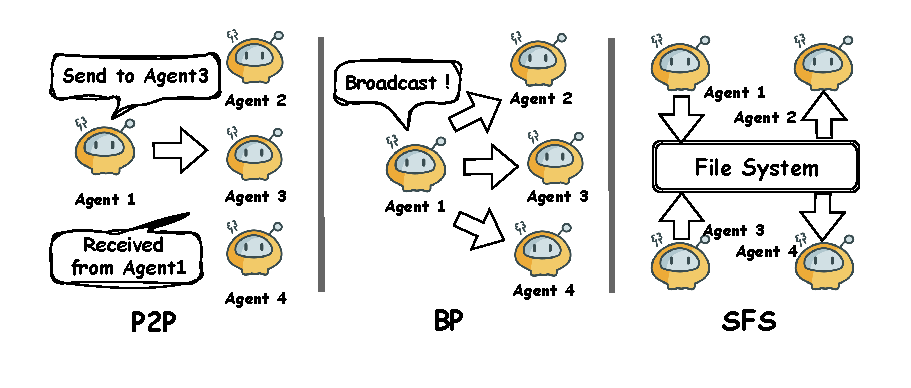
\includegraphics[width=1.0\columnwidth]{figures/protocol.pdf}
    \caption{The three communication protocols employed in \silobench{}.}
    \label{fig:protocols}
    
\end{figure}


As shown in Figure~\ref{fig:protocols}, we instantiate three protocols: \textbf{P2P}---directed messaging where agents explicitly address individual recipients; \textbf{BP}---broadcast messaging where each transmission reaches all agents simultaneously; \textbf{SFS}---indirect coordination through a shared file system. Agents retain complete autonomy in deciding what to share, with whom, and when. Detailed specifications are provided in Appendix~\ref{app:protocols}.

\paragraph{Language Model ($\mathcal{M}$).}
All $N$ agents within a configuration share the same model, isolating coordination capability from heterogeneity effects. 
We evaluate three frontier open-source models: \textbf{DeepSeek-V3.1} \citep{liu2024deepseek}, \textbf{GPT-OSS-120B} \citep{openai2025gptoss120bgptoss20bmodel}, and \textbf{Qwen3-Next-80B-A3B} \citep{yang2025qwen3technicalreport}.

\begin{tcolorbox}[colback=lightyellow!10, colframe=black!50, title=Our Experimental Setup]
\texttt{Tasks}: 30 \texttt{(10 per difficulty level)}
\\
\texttt{Scales}: 6 \texttt{(2, 5, 10, 20, 50, 100)}
\\
\texttt{Protocols}: 3 \texttt{(P2P, BP, SFS)}
\\
\texttt{Models}: 3 \texttt{(DeepSeek, GPT, Qwen)}
\end{tcolorbox}

This yields $6 \times 3 \times 3 = 54$ unique configurations and $30 \times 54 = 1{,}620$ total experiments (see Appendix~\ref{app:experiment_details} for infrastructure details). 
To disentangle coordination overhead from intrinsic task difficulty, we additionally conduct \textbf{$N{=}1$ baseline} experiments where a single agent receives the complete global input and answers directly without communication. 
We define \textbf{Relative Coordination Cost (RCC)} $= 1 - \text{SR}(N{=}k)/\text{SR}(N{=}1)$, capturing the fraction of single-agent performance lost to coordination overhead. 
The $N{=}1$ oracle represents the upper bound; \silobench{} asks whether distributed agents can approach this bound through coordination alone.

\subsection{Overall Performance}

Table~\ref{tab:overall_results} summarizes performance across all models and configurations. 
DeepSeek-V3.1 achieves a 36.9\% average success rate, followed by GPT-OSS-120B at 16.9\% and Qwen3 at 8.2\%---a 4.5$\times$ spread. 
Even the strongest model fails nearly two-thirds of the time, establishing that current LLMs cannot reliably coordinate under information silos.

\paragraph{Coordination overhead, not task difficulty, drives the performance gap.}
To confirm that failures stem from coordination rather than intrinsic task hardness, we compare multi-agent success rates against the $N{=}1$ oracle. 
Table~\ref{tab:n1_rcc} reports results for GPT-OSS-120B (trends are consistent across models). 
Even at the smallest team size ($k{=}2$), multi-agent systems already lose 15--49\% of single-agent performance, and RCC compounds steadily with scale, reaching 80--100\% at $k{=}50$ for Level-II and Level-III tasks. 
Crucially, the single-agent success rate difference between Level-I and Level-III is modest---only about 15 percentage points---yet the multi-agent gap balloons to over 18 percentage points, confirming that performance collapse is driven by coordination failure, not by the tasks themselves being harder.

\paragraph{Agents gather information but fail to integrate it.}
While RCC reveals \emph{that} coordination fails, the Partial Correctness Score (PCS) reveals \emph{where}. 
PCS measures continuous answer quality (Section~\ref{sec:metrics}), and the divergence between PCS and SR isolates the reasoning-integration stage as the bottleneck. 
At $N{\geq}50$ on Level-III tasks, SR drops to 0\% while PCS remains at 8--16\%, confirming that agents acquire partial global information but cannot synthesize it correctly.
This dissociation appears even on simpler tasks: averaged across all scales on Level-I tasks, DeepSeek-V3.1 achieves a PCS of 88.0\% yet an SR of only 62.0\% (Table~\ref{tab:overall_results}), a gap of 26 percentage points indicating that agents collectively hold nearly all required information but still fail to produce a correct final answer.

\paragraph{Performance degrades multiplicatively with scale and complexity.}
Figure~\ref{fig:difficulty} and Table~\ref{tab:scale_difficulty} show that task complexity and agent scale interact multiplicatively. DeepSeek-V3.1 drops from 62\% on Level-I to 12\% on Level-III, and Level-III tasks reach \emph{zero} success at $N{\geq}50$, while Level-I tasks remain above 40\% even at 100 agents. 
As Figure~\ref{fig:scaling} illustrates, all models degrade with agent count, and communication density \emph{decreases} at larger scales and agents become sparser in interaction precisely when denser coordination is most needed.

\begin{table*}[t]
\centering
\small
\renewcommand{\arraystretch}{1.1}
\begin{tabular}{l cc cc cc cc cc cc}
\toprule
\multirow{3}{*}{\textbf{Dimension}} 
  & \multicolumn{4}{c}{\textbf{DeepSeek-V3.1}} 
  & \multicolumn{4}{c}{\textbf{GPT-OSS-120B}} 
  & \multicolumn{4}{c}{\textbf{Qwen3-Next-80B-A3B}} \\
\cmidrule(lr){2-5}\cmidrule(lr){6-9}\cmidrule(lr){10-13}
& SR$\uparrow$ & PCS$\uparrow$ & Token$\downarrow$ & Den. 
& SR$\uparrow$ & PCS$\uparrow$ & Token$\downarrow$ & Den. 
& SR$\uparrow$ & PCS$\uparrow$ & Token$\downarrow$ & Den. \\
\midrule
\rowcolor{gray!20} \multicolumn{13}{c}{\textit{By Communication Protocol}} \\
\quad BP  & \textbf{40.4} & \textbf{50.7} & 297.3 & 0.93  
          & 14.4 & 33.1 & 148.7 & 0.78  
          & 4.5  & 12.2 & 846.9 & 0.13 \\
\quad P2P & 38.9 & 50.4 & 363.1 & 1.52  
          & \textbf{20.3} & \textbf{42.6} & 579.8 & 2.25  
          & \textbf{10.5} & \textbf{26.5} & 909.8 & 0.62 \\
\quad SFS & 31.5 & 41.0 & 308.5 & 1.13  
          & 16.0 & 34.7 & 212.8 & 0.74  
          & 9.5  & 18.7 & 864.4 & 0.21 \\
\midrule
\rowcolor{gray!20} \multicolumn{13}{c}{\textit{By Difficulty Level}} \\

\quad Level I   & \textbf{62.0} & \textbf{88.0} & 184.0 & 0.71 
                & \textbf{27.4} & \textbf{56.8} & 187.1 & 1.05 
                & \textbf{20.7} & \textbf{44.4} & 747.1 & 0.62 \\
\quad Level II  & 35.1 & 59.7 & 355.9 & 0.98 
                & 14.5 & 35.3 & 330.1 & 1.18 
                & 2.9  & 11.9 & 990.1 & 0.19 \\
\quad Level III & 11.7 & 27.9 & 439.2 & 1.93 
                & 8.8  & 22.7 & 424.2 & 1.54 
                & 1.0  & \phantom{0}1.5 & 881.6 & 0.16 \\
\midrule
\rowcolor{gray!20} \multicolumn{13}{c}{\textit{By Agent Scale}} \\

\quad N = 2  & \textbf{61.2} & \textbf{78.4} & 12.1  & 2.80 
             & \textbf{34.4} & \textbf{52.0} & 6.3   & 2.82 
             & \textbf{17.2} & \textbf{23.7} & 41.2  & 0.54 \\
\quad N = 5  & 48.5 & 68.2 & 44.2  & 1.94 
             & 28.0 & 47.9 & 30.6  & 1.78 
             & 9.1  & 15.7 & 112.4 & 0.42 \\
\quad N = 10 & 39.9 & 59.1 & 91.3  & 1.19 
             & 14.0 & 36.8 & 77.6  & 1.35 
             & 8.6  & 19.0 & 261.4 & 0.38 \\
\quad N = 20 & 33.6 & 60.2 & 211.0 & 0.72 
             & 13.2 & 37.0 & 194.1 & 0.88 
             & 7.4  & 20.1 & 549.6 & 0.35 \\
\quad N = 50 & 19.0 & 46.8 & 510.3 & 0.25 
             & 5.2  & 27.3 & 549.8 & 0.46 
             & 5.1  & 9.1  & 1466.3& 0.14 \\
\quad N = 100& 18.1 & 46.5 & 1093.8& 0.14 
             & 6.4  & 28.7 & 1024.2& 0.24 
             & 1.3  & 5.1  & 2901.1& 0.08 \\
\midrule
\textbf{Average} & \textbf{36.9} & \textbf{47.1} & 323.0 & 0.82 
                 & 16.9 & 38.3 & 313.8 & 1.01 
                 & 8.2  & 19.8 & 873.6 & 0.25 \\
\bottomrule
\end{tabular}
\caption{Overall performance summary across all models and configurations. SR = Success Rate (\%), PCS = Partial Correctness Score (\%), Token = Token Consumption (tokens/round), Den.\ = Communication Density. Best results per section in \textbf{bold}.}
\label{tab:overall_results}
\end{table*}


\begin{table*}[t]
\centering
\small
\renewcommand{\arraystretch}{1.15}
\setlength{\tabcolsep}{5pt}
\begin{tabular}{ll
  c c >{\columncolor{pink!20}}c  
  c c >{\columncolor{pink!20}}c  
  c c >{\columncolor{pink!20}}c} 
\toprule
& & \multicolumn{3}{c}{\textbf{Level I (Aggregation)}} 
& \multicolumn{3}{c}{\textbf{Level II (Mesh)}}
& \multicolumn{3}{c}{\textbf{Level III (Global Shuffle)}} \\
\cmidrule(lr){3-5}\cmidrule(lr){6-8}\cmidrule(lr){9-11}
\textbf{Scale $k$} & \phantom{x}
& SR($N$=1) & SR($N$=$k$) & RCC
& SR($N$=1) & SR($N$=$k$) & RCC
& SR($N$=1) & SR($N$=$k$) & RCC \\
\midrule
k = 2   && 96.7 & 82.0 & \cellcolor{pink!20}15.2\% & 90.0 & 62.0 & \cellcolor{pink!20}31.1\% & 80.0 & 41.0 & \cellcolor{pink!20}48.8\% \\  
k = 5   && 93.3 & 65.0 & \cellcolor{pink!20}30.3\% & 70.0 & 47.0 & \cellcolor{pink!20}32.9\% & 73.3 & 22.0 & \cellcolor{pink!20}70.0\% \\  
k = 10  && 76.7 & 51.3 & \cellcolor{pink!20}33.1\% & 73.3 & 22.0 & \cellcolor{pink!20}70.0\% & 60.0 &  9.0 & \cellcolor{pink!20}85.0\% \\  
k = 20  && 63.3 & 48.0 & \cellcolor{pink!20}24.2\% & 36.7 & 14.0 & \cellcolor{pink!20}61.8\% & 43.3 &  7.0 & \cellcolor{pink!20}83.8\% \\  
k = 50  && 33.3 & 18.0 & \cellcolor{pink!20}45.9\% & 30.0 &  6.0 & \cellcolor{pink!20}80.0\% & 26.7 &  0.0 & \cellcolor{pink!20}100\% \\    
k = 100 && 20.0 & 10.0 & \cellcolor{pink!20}50.0\% & 13.3 &  5.0 & \cellcolor{pink!20}62.4\% & 10.0 &  0.0 & \cellcolor{pink!20}100\% \\    
\bottomrule
\end{tabular}
\caption{Single-agent baseline SR (\%), multi-agent SR (\%), and Relative Coordination Cost (RCC $= 1 - \text{SR}(N{=}k)/\text{SR}(N{=}1)$) for GPT-OSS-120B across difficulty levels and scales. RCC columns (shaded) quantify the fraction of single-agent performance lost to coordination overhead. Trends are consistent across all three models; full results in Appendix~\ref{app:detailed}.}
\label{tab:n1_rcc}
\end{table*}

\begin{table}[t]
\centering
\small
\renewcommand{\arraystretch}{1.1}
\begin{tabular}{l cccccc}
\toprule
\textbf{Level} & \textbf{N=2} & \textbf{N=5} & \textbf{N=10} & \textbf{N=20} & \textbf{N=50} & \textbf{N=100} \\
\midrule
I & 85.0 & 72.0 & 68.7 & 65.7 & 38.1 & 40.6 \\
II & 61.7 & 55.3 & 28.3 & 29.5 & 17.4 & 14.3 \\
III & 36.2 & 17.2 & 10.0 & 5.7 & 0.0 & 0.0 \\
\midrule
\textbf{Avg} & 61.2 & 48.5 & 39.9 & 33.6 & 19.0 & 18.1 \\
\bottomrule
\end{tabular}
\caption{Success Rate (\%) by agent count and difficulty level for DeepSeek-V3.1 (averaged across all protocols).}
\label{tab:scale_difficulty}
\end{table}

\begin{figure*}[t]
    \centering
    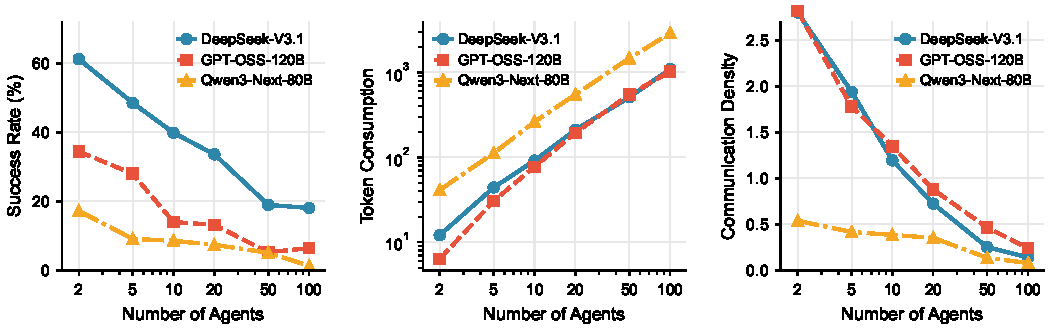
\includegraphics[width=0.95\textwidth]{figures/figure3_scaling_curves.pdf}
    \caption{Scaling behavior across agent counts. \textbf{(a)} Success rates decline for all models as team size increases, with sharp drops beyond $N=20$. \textbf{(b)} Token consumption scales roughly linearly with agent count. \textbf{(c)} Communication density decreases at scale, suggesting coordination sparsification.}
    \label{fig:scaling}
\end{figure*}

\begin{figure}[t]
    \centering
    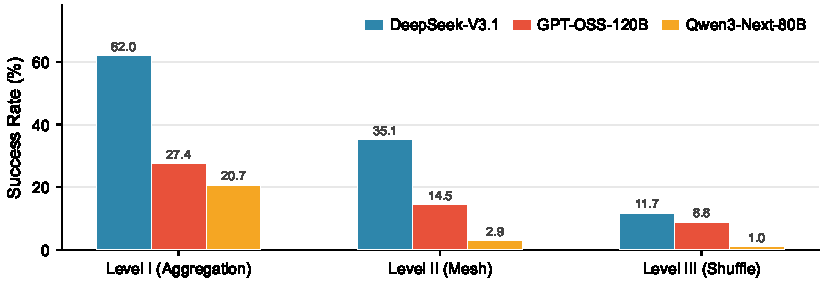
\includegraphics[width=0.95\columnwidth]{figures/difficulty_comparison.pdf}
    \caption{Success rate by difficulty level.}
    \label{fig:difficulty}
\end{figure}


\subsection{Protocol Suitability}

Having established that coordination fails broadly, we examine whether protocol choice modulates this failure. 
Figure~\ref{fig:protocol} reveals distinct model-protocol affinities. 
DeepSeek-V3.1 prefers broadcast messaging (40\% with BP vs.\ 32\% with SFS), while GPT-OSS-120B performs best with targeted communication (20\% under P2P vs.\ 14\% under BP), suggesting that protocol suitability depends on how a model balances the cognitive cost of addressing decisions against the noise of undifferentiated broadcasts. 
SFS underperforms in most cases: despite comparable information transfer volume to BP, it consistently yields lower SR, indicating that the bottleneck lies in reasoning about shared state rather than in communication volume.


\begin{figure}[ht]
    \centering
    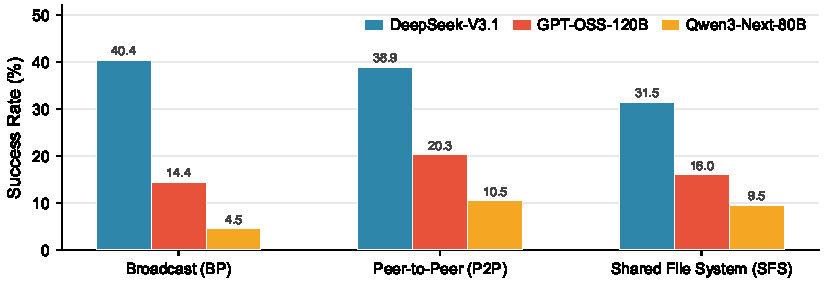
\includegraphics[width=0.95\columnwidth]{figures/protocol_comparison.pdf}
    \caption{Success rate by communication protocol.}
    \label{fig:protocol}
\end{figure}